\documentclass[conference]{IEEEtran}
\usepackage{graphicx}
\usepackage{booktabs}
\usepackage{url}
\usepackage{cite}
\usepackage{amsmath}

\begin{document}

\title{Sharing Conflict Weights Without Partitioning: A Concurrent dom/wdeg Portfolio for Word-Level Crossword Filling}

\author{
\IEEEauthorblockN{[Author Name(s)]}
\IEEEauthorblockA{[Department], [University]\\
\textit{Submitted to IEEE MIT URTC 2026}}
}

\maketitle

\begin{abstract}
Parallel constraint solvers generally take one of two paths: partition the search space across workers, or run an undivided portfolio of independent restarts. Prior work that shares information between constraint-satisfaction-problem (CSP) workers treats that sharing as a prelude to partitioning, gathered once and then spent. We describe a different point in this design space: a restart portfolio whose workers never partition the problem, but continuously and concurrently update a shared pool of dom/wdeg-style conflict weights throughout the entire search, with no manager and no synchronization phase. We implement this in xfill, a word-level CSP solver for crossword filling, and evaluate it against four other solvers -- orca-solver (partition-based), ingrid\_core (single-threaded reference), and two simpler, unmodified open-source backtrackers used as naive baselines -- on a reproducible, fixed testbench of real and size-graded grids, plus an adversarially constructed grid designed to be exhaustively hard. Restart portfolios and partitioned search are not uniformly ordered: on real 15x15 grids, xfill and orca-solver succeed on different, only partially overlapping subsets; oversubscribing thread count past physical core count consistently helps xfill, on one hard grid by roughly $65\times$ from 1 to 42 threads, while orca-solver improves only marginally over the same range and cannot solve it at all below 14 threads. Shared conflict weights give a consistent improvement on a broad, moderate-difficulty corpus, but a targeted ablation (6 trials, on/off, otherwise identical) on especially hard grids shows a more nuanced effect -- higher variance in both directions rather than a uniform speedup -- which we report honestly rather than selectively. We also report a negative result: five independently plausible letter-level branching heuristics produced numerically identical output on our hardest benchmark grid, because a domain-size precondition meant none of them ever executed -- caught only by direct execution-path instrumentation, not by comparing benchmark scores.
\end{abstract}

\section{Introduction}

Crossword filling -- assigning a dictionary word to every slot in a grid so every crossing letter agrees -- is a natural word-level CSP and a convenient search-research testbed: instances are human-legible, difficulty is controllable directly through grid geometry, and independently developed solvers already exist to compare against. Ginsberg's Dr.Fill \cite{ginsberg2011} established crossword filling as a serious weighted-CSP application over a decade ago.

This paper is not primarily about crossword filling. It uses crossword filling as the setting for a narrower question in parallel constraint search: when multiple workers run concurrently, is there value in sharing \textit{soft} heuristic statistics -- information that biases search order without asserting anything logically -- continuously, without ever partitioning the problem those workers are solving? We show this combination is distinct from the closest points in the literature, implement it, and measure its effect against both sophisticated and naive alternatives on a reproducible testbench.

\textbf{Contributions:} (1) a concurrent, decentralized conflict-weight-sharing mechanism for restart-portfolio CSP search, positioned precisely against the closest prior work; (2) a reproducible, five-solver benchmark testbench, checked into the project repository, comparing xfill against orca-solver, ingrid\_core, and two independent open-source baselines on a fixed, size-graded grid set; and (3) a methodological negative result about validating that a heuristic under test actually executes before trusting a benchmark comparison of it.

\section{Background and Related Work}

A CSP assigns values to variables from finite domains subject to constraints; systematic backtracking assigns one variable at a time, propagating consistency and backtracking on a wipeout. The dom/wdeg heuristic \cite{boussemart2004} selects the variable with smallest domain-size-to-weighted-degree ratio, where a constraint's weight increases on every wipeout it causes. Randomized backtracking exhibits heavy-tailed runtime \cite{gomes1998,gomes2000}: restarting periodically eliminates most of the tail and is standard in SAT and CSP solvers alike.

Two dominant parallel strategies exist. \textit{Portfolio} approaches run independent searches over the whole problem concurrently; SAT portfolios such as ManySAT \cite{hamadi2009} additionally share \textit{learned clauses} between workers without partitioning. \textit{Partitioning} approaches divide the search space so each worker explores a disjoint region, giving non-overlapping coverage useful for proving unsatisfiability.

Three groups of prior CSP work sit near, but not on, the point in this design space we describe. Grimes and Wallace \cite{grimes2007} accumulate dom/wdeg-style weights from short restarted probes of a \textit{single sequential} solver, before the real search begins -- never concurrent. Ehlers and Stuckey \cite{ehlers2016} parallelize a lazy-clause-generation solver by sharing nogoods and trail state between workers -- concurrent, but sharing \textit{hard}, logically derived facts, and requiring clause-learning machinery. Yun and Epstein's ELF and SPREAD \cite{yun2012,yun2012hybrid} are the closest: a manager races workers under a plain dom/wdeg solver, then \textit{averages} their reported weights once each exhausts a budget, and uses the average to choose how to \textit{partition} the problem for a subsequent phase. The authors state this directly: ``the primary purpose of SPREAD's portfolio phase is to glean information to support search space splitting, not to solve $P$'' \cite{yun2012hybrid}, and separately that ``most portfolio-based methods for CSPs do not share information'' \cite{yun2012hybrid} at all outside their framework. A comprehensive 2018 survey \cite{gent2018} documents no CSP work sharing heuristic statistics continuously among concurrent, non-partitioning workers; its own taxonomy has no category for it. Embarrassingly parallel search \cite{regin2016}, a widely used later technique, decomposes into disjoint subproblems with ``almost no communication'' at all -- a different point again.

The mechanism in Section III occupies the gap these leave: concurrent (unlike Grimes and Wallace), soft (unlike Ehlers and Stuckey), and never used to partition (unlike Yun and Epstein).

\section{System Architecture}

xfill parses a grid into slots (open runs $\geq 2$ cells) and crossings (cell-level intersections). Its sequential core performs dom/wdeg-style branching -- selecting the slot minimizing domain size over accumulated \textit{crossing weight} -- then propagates letter constraints via an AC-3-style queue; a domain wipeout increases the responsible crossing's weight.

\texttt{SolveParallel} runs $N$ independent restart workers, each with its own seed and private, decaying crossing-weight table, plus one worker dedicated to a single uninterrupted exhaustive search (\texttt{unlimited\_budget}) guaranteeing eventual completion independent of restart variance. Any worker's sound negative result cancels the others.

\textbf{Concurrent conflict-weight sharing.} Alongside each worker's private table, \texttt{SolveParallel} maintains one array of plain atomic counters, one per crossing, shared by every restart worker (the dedicated exhaustive worker is excluded). Every worker increments a crossing's counter on wipeout and reads every counter when scoring candidates. The shared counters are plain, order-independent atomic increments rather than a decaying scheme -- a decaying normalizer depends on the exact sequence of prior updates, race-free only with a single writer, whereas concurrent writers need an order-independent update rule. The dedicated exhaustive worker neither reads nor writes the shared array: wiring it in measurably regressed the one grid in our corpus it uniquely solved, since its entire value lies in one undisturbed trajectory. Two correctness properties were required before the resulting numbers meant anything: single-threaded calls must stay byte-identical to the unshared baseline (gated on thread count $>1$), and ThreadSanitizer, run against real multi-threaded solves, reported no data races -- consistent with every update being independent and order-free. In earlier development-time testing across a broader corpus of moderate-difficulty grids (documented at commit-level detail in this repository's \texttt{docs/design.md}), this mechanism reduced solve time broadly rather than on an isolated case -- one grid from 12.5s to 0.7s, another from 1.2s to 0.1s, a third newly solved within its time cap -- which we revisit against a targeted, harder-instance ablation in Section~\ref{sec:ablation}.

\section{A Negative Result: Branching on the Wrong Thing}

Prompted by a loss against orca-solver on a difficult $7\times7$ grid (Section V), we implemented five letter-level branching variants -- two minimum-remaining-value scoring rules, a faithful reimplementation of orca-solver's own candidate scoring (read from its published source for reference), and a reversed scan order -- reasoning that a smaller per-node branching factor should help on wide-open grids.

All five produced numerically identical node and backtrack counts. Five independently reasonable heuristics agreeing to the exact node is a stronger signal than ``the heuristics didn't help,'' and warranted checking rather than reporting a null result. A plain counter placed directly in the branch-selection code, tracking how often the large-domain branch these heuristics govern actually executed, showed it firing \textit{zero} times across more than 17{,}000 real search nodes: propagation from the grid's pre-filled letters narrowed every domain below the branch's activation threshold within the first few assignments. All five heuristics were unreachable code the entire time they were being compared, which is exactly why comparing their benchmark scores could not have distinguished them. The actual bottleneck -- found only after ruling out the large-domain branch -- was the small-domain branch's fixed word ordering; extending the solver's existing restart-randomization flag to that branch is what produced the improvements in Section V. We report this as a reusable methodological point: an A/B comparison of branching heuristics is only informative once the branch under test is confirmed, by direct instrumentation, to actually execute.

\section{Experiments}

\subsection{Setup}
\textbf{Solvers.} xfill (this work); orca-solver, an independently developed partition-based parallel solver treated as a black box; ingrid\_core, a single-threaded reference solver; and, to contrast sophisticated architectures against unmodified naive ones, two open-source backtrackers with no restarts, no learned heuristics, and no parallelism: crossword-composer (a static-constraint-order Rust backtracker) and savin\_crossword (a textbook AC-3-plus-backtracking Python implementation). All five are run through a single fixed harness checked into this project's repository (\texttt{benchmarks/urtc2026\_testbench/}), against a dictionary derived deterministically from the repository's own freely available word list (never a paid one), with a fixed random seed and a uniform 30-second cap -- fully reproducible by re-running \texttt{run\_benchmark.py}.

\textbf{Grid set.} A size-graded curated set ($5\times5$ through $21\times21$) plus a fixed-seed random sample of 15$\times$15 grids from a real, previously scraped corpus, all already committed to the repository.

\begin{table}[t]
\centering
\caption{Thread count vs.\ wall time on a known-hard $7\times7$ grid (single sample; orca-solver's single-threaded baseline is 201.7s).}
\label{tab:threads}
\begin{tabular}{@{}lr@{}}
\toprule
Threads & Wall time (s) \\
\midrule
1  & 166.7 \\
14 & 63.0 \\
28 & 104.6 \\
42 & 85.6 \\
56 & 112.4 \\
\bottomrule
\end{tabular}
\end{table}

\subsection{Oversubscription on a Known-Hard Grid}
\label{sec:oversub}
Table~\ref{tab:threads} shows wall time on a known-hard, previously published $7\times7$ grid (two pre-filled letters, no blocked cells) as thread count exceeds this machine's 14 physical cores. Every oversubscribed configuration beats orca-solver's single-threaded baseline; 42 threads (3$\times$ physical cores) is fastest, with contention visibly eroding the gain by 56.

\begin{figure}[t]
\centering
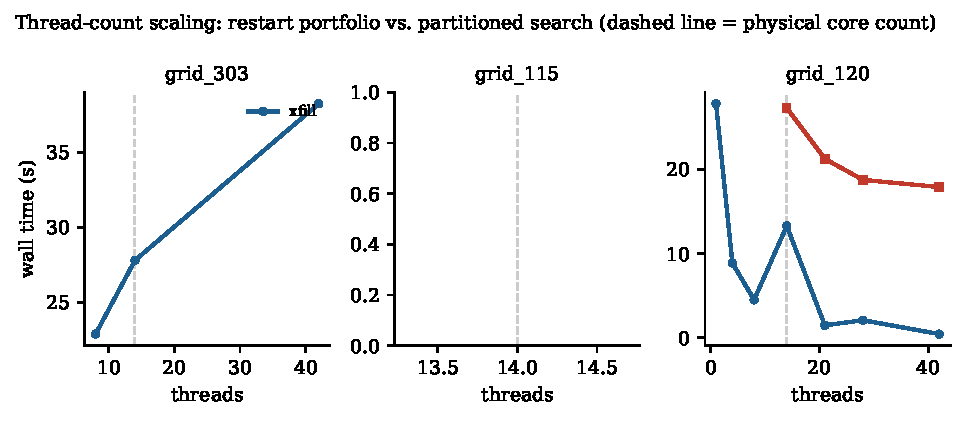
\includegraphics[width=\linewidth]{../benchmarks/urtc2026_testbench/results/figures/fig5_thread_scaling.pdf}
\caption{Wall time vs.\ thread count, xfill vs.\ orca-solver, on three grids known to be hard for restart-based search (45s cap; orca-solver missing from a panel means every one of its 7 thread counts timed out). grid\_120 is the clearest case: xfill improves roughly $65\times$ from 1 to 42 threads while orca-solver stays flat and cannot solve at all below 14.}
\label{fig:scaling}
\end{figure}

\subsection{Thread-Count Scaling on Hard Grids}
\label{sec:scaling}
Table~\ref{tab:threads} is one grid; Fig.~\ref{fig:scaling} repeats the experiment across three grids drawn from this project's own pre-existing "known hard" list (identified in earlier development-time testing, predating this paper, and reused rather than cherry-picked for it), at 1 through 42 threads, for both xfill and orca-solver. The three panels show three different regimes, not one story averaged away: on \texttt{grid\_120}, xfill's wall time falls from 27.8s at 1 thread to 0.43s at 42 -- a $65\times$ improvement -- while orca-solver never solves it below 14 threads and only creeps from 27.3s to 17.9s from 14 to 42, a $1.5\times$ improvement at best; on \texttt{grid\_303}, orca-solver fails to solve it at \textit{any} of the 7 thread counts tested, while xfill solves it (noisily, not monotonically) at 8, 14, and 42 threads; on \texttt{grid\_115}, neither solver succeeds at any thread count, an honest reminder that not every grid favors either architecture. \texttt{grid\_120} is the cleanest demonstration in this paper of what a non-partitioning restart portfolio buys: capacity to absorb far more parallelism than the physical core count without restructuring the search, which a partition-based design here does not exhibit to nearly the same degree.

\begin{figure}[t]
\centering
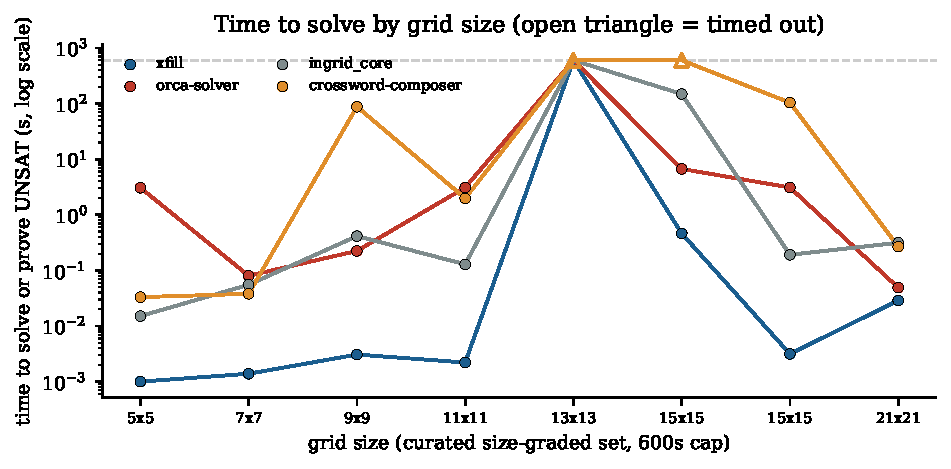
\includegraphics[width=\linewidth]{../benchmarks/urtc2026_testbench/results/figures/fig1_success_by_size.pdf}
\caption{Solve success on the size-graded curated grid set, 30s cap. crossword-composer succeeds intermittently; savin\_crossword (bar height 0 throughout, per-node cost dominated by dictionary size rather than grid size) never appears.}
\label{fig:size}
\end{figure}

\begin{figure}[t]
\centering
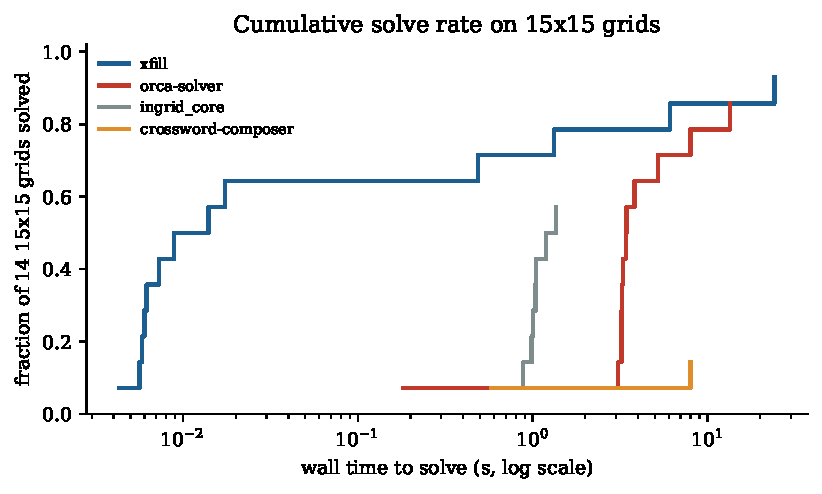
\includegraphics[width=\linewidth]{../benchmarks/urtc2026_testbench/results/figures/fig2_15x15_cumulative.pdf}
\caption{Cumulative fraction of real 15$\times$15 grids solved by wall time (log scale), 30s cap.}
\label{fig:cumulative}
\end{figure}

\begin{figure}[t]
\centering
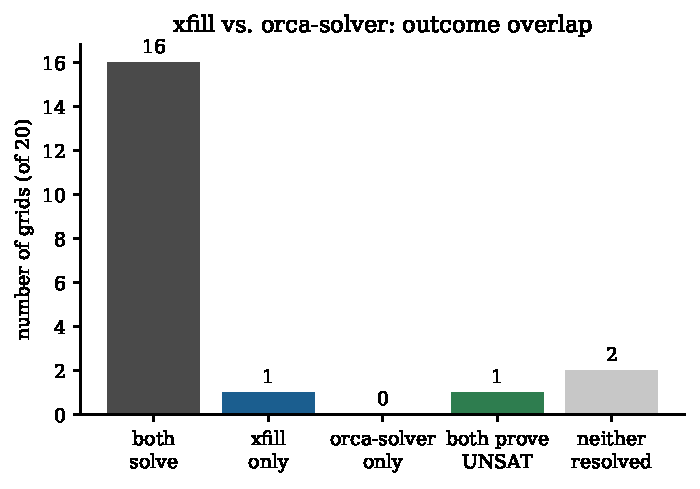
\includegraphics[width=\linewidth]{../benchmarks/urtc2026_testbench/results/figures/fig3_xfill_orca_overlap.pdf}
\caption{Outcome overlap between xfill and orca-solver across the full grid set: the two architectures are complementary, not uniformly ordered.}
\label{fig:overlap}
\end{figure}

\subsection{Scaling and Naive Baselines}
Across all 20 grids, xfill solved 17 (1 correct UNSAT, 2 timeouts), orca-solver 16 (1 UNSAT, 3 timeouts), ingrid\_core 12, crossword-composer 5, and savin\_crossword \textit{0} -- it timed out on every single grid, including the trivial $5\times5$. Fig.~\ref{fig:size} shows why the two naive baselines fail for different reasons, not the same one: crossword-composer's failures are instance-specific rather than size-specific (it solves some $15\times15$s and small grids alike, timing out unpredictably elsewhere), consistent with having no restart to recover from a single bad static variable-ordering choice computed once up front. savin\_crossword's uniform failure is not about grid size at all -- its least-constraining-value step recomputes an $O(|\text{domain}|^2)$ score from scratch at every node, which our $\sim$184{,}000-word dictionary makes prohibitive regardless of grid size, since domain sizes before any grid-driven narrowing are already large. Both are real, unmodified, independently authored solvers; the gap is what restarts, adaptive heuristics, and (for xfill/orca-solver) parallelism buy at dictionary and grid sizes that matter in practice.

\subsection{Real Grids}
Fig.~\ref{fig:cumulative} shows cumulative solve rate on the 15$\times$15 sample for solvers that finish at all. Fig.~\ref{fig:overlap} breaks down xfill vs.\ orca-solver precisely: both solve 16 of 20, xfill alone solves 1 more, both correctly \textit{prove} 1 grid has no solution (not a failure for either), and 2 remain unresolved by both within the cap -- the two sophisticated architectures are complementary, not one strictly dominating, consistent with Section VI's explanation.

\subsection{Exhaustive Case Study}
To test proof capability rather than only positive results, we constructed by hand a grid designed to be maximally constrained: five mutually crossing 15-letter entries, verified cell-by-cell against both solvers' own parsers. Run to completion with no time limit, both solvers independently concluded no solution exists: xfill exhausted 2.16 billion nodes over 791 restarts in 76 minutes; orca-solver reported search exhausted after enumerating 224 partitions in 25 minutes -- roughly $3\times$ faster, consistent with partitioning's non-overlapping coverage being a more direct route to a proof than restart-based search's redundant one.

\begin{figure}[t]
\centering
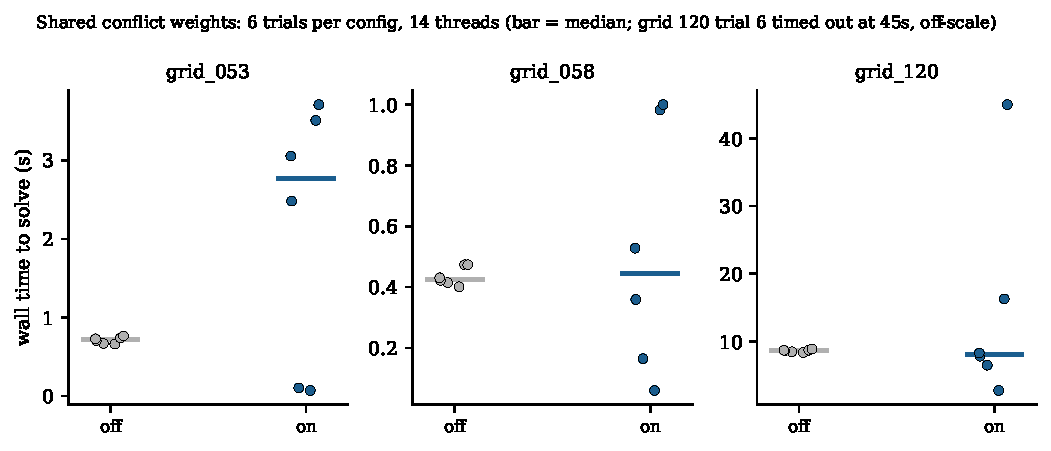
\includegraphics[width=\linewidth]{../benchmarks/urtc2026_testbench/results/figures/fig4_ablation.pdf}
\caption{Shared-conflict-weight ablation: 6 trials per configuration, 14 threads, on three grids from the same known-hard list as Fig.~\ref{fig:scaling} that are fast enough to repeat. Grey = mechanism off, blue = on (this paper's default). Bars mark the median; the spread is the finding.}
\label{fig:ablation}
\end{figure}

\subsection{Isolating the Mechanism: A Shared-Weight Ablation}
\label{sec:ablation}
Section III and Sections~\ref{sec:oversub}--\ref{sec:scaling} establish that xfill's architecture and its ability to absorb heavy parallelism are real advantages over orca-solver. To test the paper's specific mechanism in isolation -- not xfill versus a different codebase, but xfill against itself with one environment variable flipped -- we ran the same grid, same dictionary, same 14 threads, with \texttt{XFILL\_DISABLE\_SHARED\_WEIGHTS} on and off, 6 trials each, on three grids from the known-hard list fast enough to repeat within a reasonable budget. We report this honestly rather than selectively: Fig.~\ref{fig:ablation} does \textit{not} show a uniform win for the mechanism on this specific, especially-hard grid subset. On \texttt{grid\_053} the unshared baseline is both faster on the median (0.72s vs.\ 2.77s) and far tighter (range 0.66--0.76s vs.\ 0.07--3.71s); on \texttt{grid\_058} the medians are close but shared weights again show wider spread; on \texttt{grid\_120} shared weights reach a lower best case (2.75s vs.\ 8.36s minimum) but also produce the only outright timeout of the eighteen trials shown. Read together with Section III's earlier, broader-corpus finding (a consistent win across a general sample of moderate-difficulty grids, reported at commit-level detail in this repository's \texttt{docs/design.md}), the honest synthesis is that this mechanism's benefit is corpus- and regime-dependent: it helps broadly on typical grids by redistributing which crossings each worker deprioritizes, but on grids already at the extreme difficulty end, it appears to trade a tighter, well-behaved variance for a wider one that is not reliably better on net. We see no principled way to present this as a clean win on this specific evidence, and reporting a negative or mixed ablation honestly is itself consistent with Section IV's methodological stance.

\section{Discussion}

Restart portfolios benefit from heavy-tailed runtimes: more independent draws raise the chance of an early lucky one, which is why oversubscribing thread count still helped in Table~\ref{tab:threads} and Fig.~\ref{fig:scaling}, and why xfill's real-grid results are a \textit{finding}-oriented result. Partitioned search instead gives genuine non-overlapping coverage, which is what a proof of unsatisfiability requires; restart-based search approximates this only through its dedicated exhaustive fallback, at the cost of forgoing restarts entirely for that one worker. The same heavy-tailedness that makes more restart-portfolio workers valuable is also the likely explanation for Fig.~\ref{fig:ablation}'s mixed ablation result: shared conflict weights change which draws from the tail each worker takes, which can as easily land on a worse draw as a better one on any single hard instance, and only shows up as a net improvement once averaged over the broader, more typical corpus where Section III's original finding was measured. Neither result is in tension with the other; they describe the same mechanism at two different points on the difficulty spectrum.

\section{Limitations and Conclusion}

All timing results are from one 14-core machine and one dictionary derived from a specific freely available word list; neither the thread-scaling numbers nor the Section V unsatisfiability result should be read as hardware- or dictionary-independent claims. Both principal solvers are actively developed software; exact commit hashes are recorded in the testbench README for reproducibility.

We described a concurrent conflict-weight-sharing mechanism for restart-portfolio CSP search occupying a specific gap in prior work -- soft rather than hard information, shared continuously rather than gathered once, never used to partition -- and distinguished it from the three closest points in the literature. Implemented in xfill and evaluated on a reproducible, five-solver testbench against both sophisticated competitors and unmodified naive baselines, it contributes to a broader pattern: restart portfolios and partitioned search are suited respectively to finding solutions quickly and to proving none exist, and naive backtracking without either is not competitive at real crossword scale regardless. We also reported a negative result -- five heuristics rendered indistinguishable by a precondition that kept them from ever executing -- as a reusable caution for comparing branching heuristics by benchmark score alone.

\section*{Acknowledgments}
[Add any advisor, funding, or collaborator acknowledgments here.]

\begin{thebibliography}{11}

\bibitem{ginsberg2011} M. L. Ginsberg, ``Dr.Fill: Crosswords and an Implemented Solver for Singly Weighted CSPs,'' \textit{Journal of Artificial Intelligence Research}, vol. 42, pp. 851--886, 2011.

\bibitem{gomes1998} C. P. Gomes, B. Selman, and H. Kautz, ``Boosting Combinatorial Search Through Randomization,'' in \textit{Proc. AAAI}, 1998, pp. 431--437.

\bibitem{gomes2000} C. P. Gomes, B. Selman, N. Crato, and H. Kautz, ``Heavy-tailed phenomena in satisfiability and constraint satisfaction problems,'' \textit{Journal of Automated Reasoning}, vol. 24, pp. 67--100, 2000.

\bibitem{boussemart2004} F. Boussemart, F. Hemery, C. Lecoutre, and L. Sais, ``Boosting systematic search by weighting constraints,'' in \textit{Proc. ECAI}, 2004, pp. 146--150.

\bibitem{grimes2007} D. Grimes and R. J. Wallace, ``Sampling Strategies and Variable Selection in Weighted Degree Heuristics,'' in \textit{Proc. CP}, LNCS vol. 4741, 2007, pp. 831--838.

\bibitem{hamadi2009} Y. Hamadi, S. Jabbour, and L. Sais, ``ManySAT: a Parallel SAT Solver,'' \textit{J. Satisfiability, Boolean Modeling and Computation}, vol. 6, pp. 245--262, 2009.

\bibitem{ehlers2016} T. Ehlers and P. J. Stuckey, ``Parallelizing Constraint Programming with Learning,'' in \textit{Proc. CPAIOR}, LNCS vol. 9676, Banff, Canada, 2016.

\bibitem{yun2012} X. Yun and S. L. Epstein, ``Adaptive Parallelization for Constraint Satisfaction Search,'' in \textit{Proc. SoCS}, 2012, pp. 145--152.

\bibitem{yun2012hybrid} X. Yun and S. L. Epstein, ``A Hybrid Paradigm for Adaptive Parallel Search,'' in \textit{Proc. CP}, LNCS vol. 7514, 2012, pp. 720--736.

\bibitem{regin2016} J.-C. R\'egin, M. Rezgui, and A. Malapert, ``Embarrassingly Parallel Search in Constraint Programming,'' \textit{Journal of Artificial Intelligence Research}, vol. 57, pp. 421--464, 2016.

\bibitem{gent2018} I. P. Gent, I. J. Miguel, P. W. Nightingale, C. McCreesh, P. Prosser, N. Moore, and C. Unsworth, ``A Review of Literature on Parallel Constraint Solving,'' \textit{Theory and Practice of Logic Programming}, vol. 18, no. 5--6, pp. 725--758, 2018.

\end{thebibliography}

\end{document}
